32. $y=1-|x-2|=\begin{cases} 1-x+2=3-x,\ x\geqslant2,\\ 1+x-2=x-1,\ x<2.\end{cases}$
$$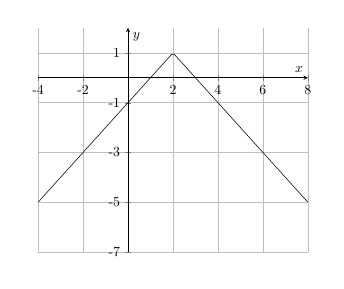
\begin{tikzpicture}[scale=0.5]
\begin{axis}[
    axis lines = middle,
    grid=major,
    legend pos={south west},
    xlabel = {$x$},
    ylabel = {$y$},
    ymin=-7,
    ymax=2,
    xtick={ -4, -2, 2,4,6,8},
    xticklabels={ -4, -2, 2,4,6,8},
    ytick={-7,-5,-3, 1, -1},
    yticklabels={-7,-5,-3, 1, -1}            ]
	\addplot[domain=-4:8, samples=100, color=black] {1-abs(x-2)};
%\addplot[domain=-3.1:2.5, samples=100, color=red] {70*abs(1-2*abs(abs(x)-2))-10*x^2+10*x-70};
	%\addlegendentry{$\text{Рис. 1}$};
\end{axis}
\end{tikzpicture}$$
